
\section{David Tong QFT PS3}
\subsection{3-to-3 Scattering in \texorpdfstring{$\phi^4$}{phi4} Theory, Q1}
A real scalar field with $\phi^4$ interaction has the Lagrangian
\begin{equation}
    \mathcal{L} = \frac{1}{2}\partial_\mu\phi\,\partial^\mu\phi - \frac{1}{2}m^2\phi^2 - \frac{\lambda}{4!}\phi^4.
\end{equation}
Use Dyson's formula and Wick's theorem to show that the leading order contribution to 3-particle $\to$ 3-particle scattering includes the amplitude
\usetikzlibrary{decorations.markings, arrows.meta}

\begin{equation}
    \vcenter{\hbox{
    \begin{tikzpicture}[
  thick,
  every node/.style={font=\small},
  momarrow/.style={-{Stealth[length=2.2mm]}, thin}
]
  % --- Vertices (just coordinates, no markers) ---
  \coordinate (a) at (0,0);
  \coordinate (b) at (3,0);

  % --- External legs, fanning out symmetrically ---
  \coordinate (i1) at (-1.8, 1.5);
  \coordinate (i2) at (-2.4, 0);
  \coordinate (i3) at (-1.8,-1.5);
  \coordinate (f1) at ( 4.8, 1.5);
  \coordinate (f2) at ( 5.4, 0);
  \coordinate (f3) at ( 4.8,-1.5);

  % --- Diagram lines ---
  \draw (i1) -- (a);
  \draw (i2) -- (a);
  \draw (i3) -- (a);
  \draw (a)  -- (b);
  \draw (b)  -- (f1);
  \draw (b)  -- (f2);
  \draw (b)  -- (f3);

  % --- Momentum arrows: short, parallel, offset to the OUTER side of each line.
  %     Each arrow runs from 20% to 80% along its line, shifted perpendicularly. ---

  % p1: i1 -> a, offset up-right (outside upper-left wedge)
  \draw[momarrow] ($(i1)!0.2!(a) +(0.20, 0.24)$) -- ($(i1)!0.8!(a) +(0.20, 0.24)$)
    node[midway, above right, inner sep=1pt] {$p_1$};

  % p2: i2 -> a, horizontal, offset up
  \draw[momarrow] ($(i2)!0.2!(a) +(0, 0.28)$) -- ($(i2)!0.8!(a) +(0, 0.28)$)
    node[midway, above] {$p_2$};

  % p3: i3 -> a, offset down-right (outside lower-left wedge)
  \draw[momarrow] ($(i3)!0.2!(a) +(0.20,-0.24)$) -- ($(i3)!0.8!(a) +(0.20,-0.24)$)
    node[midway, below right, inner sep=1pt] {$p_3$};


  % p4: b -> f1, offset up-left (outside upper-right wedge)
  \draw[momarrow] ($(b)!0.2!(f1) +(-0.20, 0.24)$) -- ($(b)!0.8!(f1) +(-0.20, 0.24)$)
    node[midway, above left, inner sep=1pt] {$p_1'$};

  % p5: b -> f2, horizontal, offset up
  \draw[momarrow] ($(b)!0.2!(f2) +(0, 0.28)$) -- ($(b)!0.8!(f2) +(0, 0.28)$)
    node[midway, above] {$p_2'$};

  % p6: b -> f3, offset down-left (outside lower-right wedge)
  \draw[momarrow] ($(b)!0.2!(f3) +(-0.20,-0.24)$) -- ($(b)!0.8!(f3) +(-0.20,-0.24)$)
    node[midway, below left, inner sep=1pt] {$p_3'$};
\end{tikzpicture}
    }} = (-i\lambda)^2\,\frac{i}{(p_1+p_2+p_3)^2 - m^2}
\end{equation}
Check that this result is consistent with the Feynman rules for the theory. What other diagrams also contribute to this process?
\begin{solution}
    The Dyson equation is 
    \begin{equation}
        \bra{\Omega}T\phi(x_1)\cdots\phi(x_6)\ket{\Omega} = \frac{\bra{0}T\phi(x_1)\cdots\phi(x_6)e^{i\int d^4x\mathcal{L}_\text{int}}\ket{0}}{\bra{0}Te^{i\int d^4x\mathcal{L}_\text{int}}\ket{0}}.
    \end{equation}
    We shall first expand the exponential of the interaction Lagrangian, giving
    \begin{equation}
        e^{i\int d^4x\mathcal{L}_\text{int}} = 1 -\frac{i\lambda}{4!}\int d^4x\,\phi^4(x) + \frac{1}{2}\left(-\frac{i\lambda}{4!}\right)^2\int d^4x\int d^4y \,\phi^4(x)\phi^4(y) +\mathcal{O}(\lambda^3).
    \end{equation}
    Since all the disconnected diagrams including vacuum bubbles are cancelled by the denominator in the Dyson equation, we consider only the connected ones. Therefore, the leading order contribution comes from $\lambda^2$. In particular, we consider all the possible connected contractions of 
    \begin{equation}
        \bra{0}T\phi_1\phi_2\phi_3\phi_4\phi_5\phi_6\phi_x^4\phi_y^4\ket{0},
    \end{equation}
    where we denote $\phi_1 \equiv \phi(x_1)$ and $\phi_x\equiv\phi(x)$. Note that the only connected diagram with distinct topology we can construct from this is
    \begin{equation}
        D_{1x}D_{2x}D_{3x}D_{xy}D_{y4}D_{y5}D_{y6}.
    \end{equation}
    Now, we need to count the prefactor of this diagram. First, we can choose three $\phi_i$ (assuming they are distinguishable) to contract with four $\phi_x$, and since the scalar particles are identical we can permute them, which gives
    \begin{equation}
        \begin{pmatrix}
            4\\3
        \end{pmatrix}\times 3!.
    \end{equation}
    The same applies for the rest three fields and the $y$ vertex. Finally, we can interchange $x$ and $y$. Hence, the prefactor is
    \begin{equation}
        \begin{pmatrix}
            4\\3
        \end{pmatrix}\times 3! \times\begin{pmatrix}
            4\\3
        \end{pmatrix}\times 3!\times2 = 1152 = 2\times(4!)^2.
    \end{equation}
    Therefore, the vacuum expectation value is given by
    \begin{equation}
        \bra{\Omega}T\phi(x_1)\cdots\phi(x_6)\ket{\Omega} = (-i\lambda)^2\int d^4x\int d^4yD_{1x}D_{2x}D_{3x}D_{xy}D_{y4}D_{y5}D_{y6},
    \end{equation}
    where
    \begin{equation}
        D_{ij} = \int\frac{d^4 p }{(2\pi)^4}\frac{ie^{-ip\cdot(x_i-x_j)}}{p^2-m^2+i\epsilon}.
    \end{equation}
    Using the LSZ reduction formula,
    \begin{equation}
       \begin{aligned}
                \bra{f}S\ket{i} = \biggr[ i\int d^4x_1e^{-ip_1x_1}(\square_1+m^2) \biggr] \cdots \biggr[ i\int d^4x_ne^{ip_nx_n}(\square_n+m^2) \biggr]\\
                \times \bra{\Omega}T\{\phi(x_1) \dots \phi(x_n)\}\ket{\Omega},
    \end{aligned}\tag{5.13} 
    \end{equation}
    and note that integrating over the position integrals gives a $\delta$-function fixing the external momenta. Therefore, we find
    \begin{equation}
    \begin{aligned}
        \bra{f}S\ket{i} &= (-i\lambda)^2\int d^4x \int d^4y\int\frac{d^4p}{(2\pi)^4}\frac{ie^{-ip\cdot(x-y)}}{p^2-m^2+i\epsilon}e^{i(p_1+p_2+p_3)\cdot x}e^{-i(p_1'+p_2'+p_3')\cdot y} \\
        &=(-i\lambda)^2\frac{i}{(p_1+p_2+p_3)^2-m^2+i\epsilon}(2\pi)^4\delta(p_1+p_2+p_3 - p_1'-p_2'-p_3').
    \end{aligned} 
    \end{equation}
    Now, recall 
    \begin{equation}
        \bra{f}S\ket{i} = (2\pi)^4i\mathcal{M}\delta\left(\sum_ip_i\right),
    \end{equation}
    we find
    \begin{equation}
        i\mathcal{M}= (-i\lambda)^2\,\frac{i}{(p_1+p_2+p_3)^2 - m^2}.
    \end{equation}
    
\end{solution}

\subsection{Vacuum Bubbles and the Exponential Formula, Q2}

Examine $\langle 0|S|0\rangle$ to order $\lambda^2$ in $\phi^4$ theory. Identify the different diagrams with the different contributions arising from an application of Wick's theorem. Confirm that to order $\lambda^2$, the combinatoric factors work out so that the vacuum to vacuum amplitude is given by the exponential of the sum of distinct vacuum bubble types,
\begin{equation}
    \langle 0|S|0\rangle = \exp\left(
    \vcenter{\hbox{
    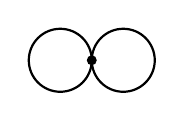
\begin{tikzpicture}[thick]
      \coordinate (a) at (0,0);
      \draw (a)++(-0.4,0) circle(0.4);
      \draw (a)++(+0.4,0) circle(0.4);
      \fill (a) circle(1.8pt);
    \end{tikzpicture}}}
    \;+\;
    \vcenter{\hbox{
    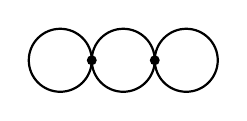
\begin{tikzpicture}[thick]
      \coordinate (p) at (0.4,0);
      \coordinate (q) at (1.2,0);
      \draw (p)++(-0.4,0) circle(0.4);
      \draw (p)++(+0.4,0) circle(0.4);
      \draw (q)++(0.4,0) circle(0.4);
      \fill (p) circle(1.8pt);
      \fill (q) circle(1.8pt);
    \end{tikzpicture}}}
    \;+\;
    \vcenter{\hbox{
    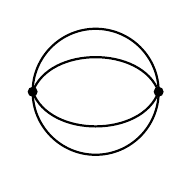
\begin{tikzpicture}[thick]
      \coordinate (r) at (0,0);
      \coordinate (s) at (1.6,0);
      \draw (r) to[bend left=70]  (s);
      \draw (r)++(0.8,0) circle(0.8);
      \draw (r) to[bend right=70] (s);
      \fill (r) circle(1.8pt);
      \fill (s) circle(1.8pt);
    \end{tikzpicture}}}
    \;+\;\cdots\right).
\end{equation}

\begin{solution}
    Here, the free vacuum expectation value of the $S$-matrix is meant by
    \begin{equation}
        \bra{0}S\ket{0} = \bra{0}Te^{i\int d^4\mathcal{L}_\text{int}}\ket{0}.
    \end{equation}
    Expanding it to second order in $\lambda$, we find
    \begin{equation}
        \bra{0}S\ket{0} = 1 + \left(\frac{-i\lambda}{4!}\right)\int d^4x \bra{0}T\phi^4(x)\ket{0} + \frac{1}{2}\left(\frac{-i\lambda}{4!}\right)^2\int d^4x\int d^4y \bra{0}T\phi^4(x)\phi^4(y)\ket{0} + \mathcal{O}(\lambda^3).
    \end{equation}
    Let us consider it term by term. The second term has only one possible contraction,
    \begin{equation}
        \left(\frac{-i\lambda}{4!}\right)\int d^4x  \bra{0}T\phi^4(x)\ket{0}  = -i\lambda\frac{1}{8}\int d^4x\,D(0)^2 =  
    \vcenter{\hbox{
    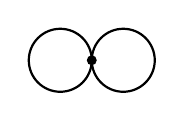
\begin{tikzpicture}[thick]
      \coordinate (a) at (0,0);
      \draw (a)++(-0.4,0) circle(0.4);
      \draw (a)++(+0.4,0) circle(0.4);
      \fill (a) circle(1.8pt);
    \end{tikzpicture}}}\;,
    \end{equation}
    where the factor $3$ comes from the three different ways of pairing the four fields. This gives a symmetry factor of $S=4!/3 = 8$ as expected (two loops and swapping the two loops).
    
    The third term is more interesting. There are three different diagrams from this amplitude. First, one could consider the contraction
    \begin{equation}
        \frac{1}{2}\left(\frac{-i\lambda}{4!}\right)^2\int d^4x\int d^4y \,3^2D(x-x)^2D(y-y)^2 =\frac{(-i\lambda)^2}{2\cdot 8^2}\int d^4x\int D(0)^4 = \frac{1}{2}\left(
        \vcenter{\hbox{
    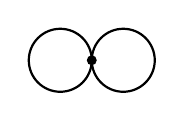
\begin{tikzpicture}[thick]
      \coordinate (a) at (0,0);
      \draw (a)++(-0.4,0) circle(0.4);
      \draw (a)++(+0.4,0) circle(0.4);
      \fill (a) circle(1.8pt);
    \end{tikzpicture}}}\,\,\right)^2.
    \end{equation}
    The next possible contraction is
    \begin{equation}
        \frac{1}{2}\left(\frac{-i\lambda}{4!}\right)^2\int d^4x\int d^4y \,2\cdot 6^2 D(0)^2D(x-y)^2 = 
        \vcenter{\hbox{
    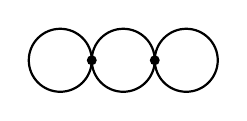
\begin{tikzpicture}[thick]
      \coordinate (p) at (0.4,0);
      \coordinate (q) at (1.2,0);
      \draw (p)++(-0.4,0) circle(0.4);
      \draw (p)++(+0.4,0) circle(0.4);
      \draw (q)++(0.4,0) circle(0.4);
      \fill (p) circle(1.8pt);
      \fill (q) circle(1.8pt);
    \end{tikzpicture}}}\,\,.
    \end{equation}
    The $6^2$ comes from choosing two $\phi(x)$ to contract with $\phi(y)$, and two $\phi(y)$ to go to $\phi(x)$. Another factor of $2$ comes from pairing the $\phi(x)$ and $\phi(y)$ chosen. This results in a symmetry factor of $S = 2\cdot(4!)^2/(2\cdot6^2) = 16$ (two loops, two permuted internal lines, and swap $x$ and $y$).
    Finally, the last contraction is
    \begin{equation}
        \frac{1}{2}\left(\frac{-i\lambda}{4!}\right)^2\int d^4x\int d^4y \, 4!D(x-y)^4 = 
        \vcenter{\hbox{
    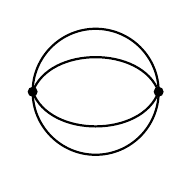
\begin{tikzpicture}[thick]
      \coordinate (r) at (0,0);
      \coordinate (s) at (1.6,0);
      \draw (r) to[bend left=70]  (s);
      \draw (r)++(0.8,0) circle(0.8);
      \draw (r) to[bend right=70] (s);
      \fill (r) circle(1.8pt);
      \fill (s) circle(1.8pt);
    \end{tikzpicture}}}\,\,,
    \end{equation}
    where the combinatoric factor came from the same reason as before. This gives a symmetry factor of $S = 2\cdot(4!)^2/4! = 48$ (four permuted internal lines and swapping the two vertices). Therefore, we have computed the perturbative expansion of the free vacuum expectation value of the $S$-matrix. That is
    \begin{equation}
        \bra{0}S\ket{0} = \vcenter{\hbox{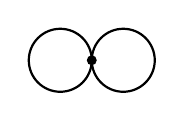
\begin{tikzpicture}[thick]
      \coordinate (a) at (0,0);
      \draw (a)++(-0.4,0) circle(0.4);
      \draw (a)++(+0.4,0) circle(0.4);
      \fill (a) circle(1.8pt);
    \end{tikzpicture}}}
    \;+\;
    \vcenter{\hbox{
    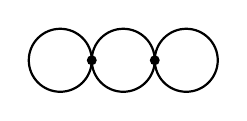
\begin{tikzpicture}[thick]
      \coordinate (p) at (0.4,0);
      \coordinate (q) at (1.2,0);
      \draw (p)++(-0.4,0) circle(0.4);
      \draw (p)++(+0.4,0) circle(0.4);
      \draw (q)++(0.4,0) circle(0.4);
      \fill (p) circle(1.8pt);
      \fill (q) circle(1.8pt);
    \end{tikzpicture}}}
    \;+\;
    \vcenter{\hbox{
    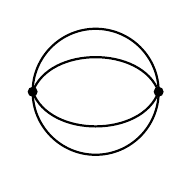
\begin{tikzpicture}[thick]
      \coordinate (r) at (0,0);
      \coordinate (s) at (1.6,0);
      \draw (r) to[bend left=70]  (s);
      \draw (r)++(0.8,0) circle(0.8);
      \draw (r) to[bend right=70] (s);
      \fill (r) circle(1.8pt);
      \fill (s) circle(1.8pt);
    \end{tikzpicture}}}
    \;+\;\frac{1}{2}
    \left(
        \vcenter{\hbox{
    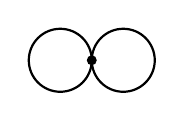
\begin{tikzpicture}[thick]
      \coordinate (a) at (0,0);
      \draw (a)++(-0.4,0) circle(0.4);
      \draw (a)++(+0.4,0) circle(0.4);
      \fill (a) circle(1.8pt);
    \end{tikzpicture}}}\,\,\right)^2
    \; + \cdots.
    \end{equation}
    
\end{solution}

\subsection{$O(3)$ Scalar Field Theory, Q3}

Consider the Lagrangian for 3 scalar fields $\phi_i$, $i=1,2,3$, given by
\begin{equation}
    \mathcal{L} = \sum_{i=1}^{3}\frac{1}{2}(\partial_\mu\phi_i)(\partial^\mu\phi_i) - \frac{1}{2}m^2\left(\sum_{i=1}^{3}\phi_i^2\right) - \frac{\lambda}{8}\left(\sum_{i=1}^{3}\phi_i^2\right)^2
\end{equation}
Show that the Feynman propagator for the free field theory (i.e.\ $\lambda=0$) is of the form
\begin{equation}
    \langle 0|T\phi_i(x)\phi_j(y)|0\rangle = \delta_{ij}D_F(x-y)
\end{equation}
where $D_F(x-y)$ is the usual scalar propagator. Write down the Feynman rules of the theory. Compute the amplitude for the scattering $\phi_i\phi_j\to\phi_k\phi_l$ to lowest order in $\lambda$.

\begin{solution}
    The Feynman propagator
    \begin{equation}
        \bra{0}T\phi_i(x_1)\phi_j(x_2)\ket{0}
    \end{equation}
    vanishes for $i\neq j$. For $i=j$, it is simply the ordinary free scalar theory. Therefore, we must have
    \begin{equation}
        \langle 0|T\phi_i(x)\phi_j(y)|0\rangle = \delta_{ij}D_F(x-y).
    \end{equation}
    The momentum space Feynman rules of the theory is 
    \begin{equation}
        \vcenter{\hbox{
        \begin{tikzpicture}[
  thick,
  every node/.style={font=\small},
  momarrow/.style={-{Stealth[length=2.2mm]}, thin}
]
            \coordinate (i1) at (1,0);
            \coordinate (a) at (-1,0);
            \draw (a) -- (i1);
              \draw[momarrow] ($(a)!0.2!(i1) +(0.05, 0.24)$) -- ($(a)!0.8!(i1) +(-0.05, 0.24)$)
                node[midway, above] {$p$};
            \node at (2.5,0) {$=\dfrac{i\delta_{ij}}{p^2-m^2+i\epsilon},$};
        \end{tikzpicture}
        }}
    \end{equation}
    and
    \begin{equation}
         \vcenter{\hbox{\begin{tikzpicture}[thick]
  \coordinate (v) at (0,0);
  \fill (v) circle (2pt);
  \coordinate (i1) at (-1.4,  1.4);
  \coordinate (i2) at (-1.4, -1.4);
  \coordinate (f1) at ( 1.4,  1.4);
  \coordinate (f2) at ( 1.4, -1.4);
  \draw (i1) -- (v);  \draw (i2) -- (v);
  \draw (f1) -- (v);  \draw (f2) -- (v);
  \node at (-1.7,  1.7) {$\phi_i$};
  \node at (-1.7, -1.7) {$\phi_j$};
  \node at ( 1.7,  1.7) {$\phi_k$};
  \node at ( 1.7, -1.7) {$\phi_l$};
  \node at (5, 0) {$= -i\lambda\,(\delta_{ij}\delta_{kl} + \delta_{ik}\delta_{jl} + \delta_{il}\delta_{jk}),$};
\end{tikzpicture}}}
    \end{equation}
    where the $\delta$'s come from contracting $\phi_a^2\phi_b^2$ with the external external fields forcing them to pair up.

    The scattering amplitude $\phi_i\phi_j \to \phi_k\phi_l$ to first order is simply given by
    \begin{equation}
        i\mathcal{M} = -i\lambda\,(\delta_{ij}\delta_{kl} + \delta_{ik}\delta_{jl} + \delta_{il}\delta_{jk}).
    \end{equation}
\end{solution}

\subsection{Yukawa Theory Scattering Amplitudes, Q4}

The Lagrangian for Yukawa theory is given by
\begin{equation}
    \mathcal{L} = \tfrac{1}{2}(\partial\phi)^2 - \tfrac{1}{2}\mu^2\phi^2 + \bar\psi(i\slashed{\partial}-m)\psi - \lambda\phi\bar\psi\psi.
\end{equation}

\textbf{a)} Consider $\psi\psi\to\psi\psi$ scattering, with the initial and final states given by
\begin{align}
    |i\rangle &= \sqrt{4E_{\mathbf{p}}E_{\mathbf{q}}}\,b^{s\dagger}_{\mathbf{p}}\,b^{r\dagger}_{\mathbf{q}}\,|0\rangle\\
    |f\rangle &= \sqrt{4E_{\mathbf{p}'}E_{\mathbf{q}'}}\,b^{s'\dagger}_{\mathbf{p}'}\,b^{r'\dagger}_{\mathbf{q}'}\,|0\rangle.
\end{align}
Show using Dyson's formula and Wick's theorem that the scattering amplitude at order $\lambda^2$ is given by
\begin{equation}
    \mathcal{M} = (-i\lambda)^2\left(\frac{[\bar{u}^{s'}(\mathbf{p}')\cdot u^s(\mathbf{p})]\,[\bar{u}^{r'}(\mathbf{q}')\cdot u^r(\mathbf{q})]}{(p'-p)^2-\mu^2} - \frac{[\bar{u}^{s'}(\mathbf{p}')\cdot u^r(\mathbf{q})]\,[\bar{u}^{r'}(\mathbf{q}')\cdot u^s(\mathbf{p})]}{(q'-p)^2-\mu^2}\right).
\end{equation}
Draw the two Feynman diagrams that correspond to these two terms.

\textbf{b)} Consider now $\psi\bar\psi\to\psi\bar\psi$ scattering, with initial and final states given by
\begin{align}
    |i\rangle &= \sqrt{4E_{\mathbf{p}}E_{\mathbf{q}}}\,b^{s\dagger}_{\mathbf{p}}\,c^{r\dagger}_{\mathbf{q}}\,|0\rangle\\
    |f\rangle &= \sqrt{4E_{\mathbf{p}'}E_{\mathbf{q}'}}\,b^{s'\dagger}_{\mathbf{p}'}\,c^{r'\dagger}_{\mathbf{q}'}\,|0\rangle.
\end{align}
Show that the amplitude is this time given by
\begin{equation}
    \mathcal{M} = -(-i\lambda)^2\left(\frac{[\bar{u}^{s'}(\mathbf{p}')\cdot u^s(\mathbf{p})]\,[\bar{v}^r(\mathbf{q})\cdot v^{r'}(\mathbf{q}')]}{(p-p')^2-\mu^2} - \frac{[\bar{v}^r(\mathbf{q})\cdot u^s(\mathbf{p})]\,[\bar{u}^{s'}(\mathbf{p}')\cdot v^{r'}(\mathbf{q}')]}{(p+q)^2-\mu^2}\right).
\end{equation}
(Be careful with minus signs!!). What are the Feynman diagrams that now contribute?

\begin{solution}
    The momentum space Feynmam rule is given by
    \begin{equation}
        \vcenter{\hbox{
        \begin{tikzpicture}[
          thick,
          every node/.style={font=\small},
          momarrow/.style={-{Stealth[length=2.2mm]}, thin}
        ]
            \coordinate (i1) at (1,0);
            \coordinate (a) at (-1,0);
            \draw (a) -- (i1);
              \draw[momarrow] ($(a)!0.2!(i1) +(0.05, 0.24)$) -- ($(a)!0.8!(i1) +(-0.05, 0.24)$)
                node[midway, above] {$k$};
            \node at (2.5,0) {$=\dfrac{i}{k^2-\mu^2+i\epsilon},$};
        \end{tikzpicture}
        }}
    \end{equation}
    \begin{equation}
        \vcenter{\hbox{
        \begin{tikzpicture}[
          thick,
          every node/.style={font=\small},
          fermion/.style={postaction={decorate},
            decoration={markings, mark=at position 0.55 with {\arrow{Stealth}}}},
        ]
            \coordinate (a) at (-1, 0);
            \coordinate (b) at ( 1, 0);
            \draw[fermion] (a) -- (b);
            \node[above] at (0, 0) {$p$};
            \node at (2.5, 0) {$=\dfrac{i(\slashed{p}+m)}{p^2-m^2+i\epsilon},$};
        \end{tikzpicture}
        }}
    \end{equation}
    and
    \begin{equation}
        \vcenter{\hbox{
        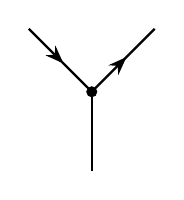
\begin{tikzpicture}[thick,
          every node/.style={font=\small},
          fermion/.style={postaction={decorate},
            decoration={markings, mark=at position 0.55 with {\arrow{Stealth}}}},
        ]
          \coordinate (v)   at ( 0,    0);
          \coordinate (vi1) at (-0.8,  0.8);
          \coordinate (vf1) at ( 0.8,  0.8);
          \coordinate (vs1) at ( 0,   -1.0);
          \draw[fermion] (vi1) -- (v);
          \draw[fermion] (v)   -- (vf1);
          \draw          (v)   -- (vs1);
          \fill (v) circle (2pt);
        \end{tikzpicture}
        }} = -i\lambda.
    \end{equation}
    \textbf{a)} Since we start with two fermions, only $u$- and $t$- channels contribute to the amplitude. The $t$-channel amplitude gives
    \begin{equation}
        i\mathcal{M}_t =
        \vcenter{\hbox{
        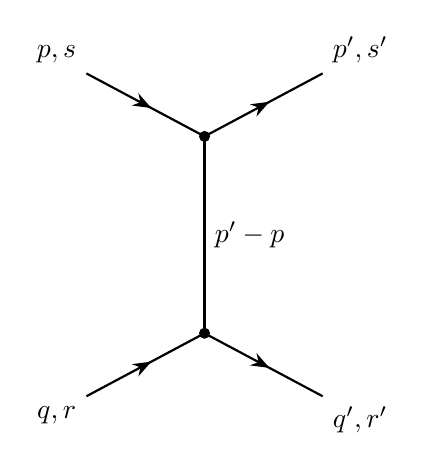
\begin{tikzpicture}[thick,
          fermion/.style={postaction={decorate},
            decoration={markings, mark=at position 0.55 with {\arrow{Stealth}}}},
        ]
          \coordinate (a)  at ( 0,  0);
          \coordinate (b)  at ( 0, -2.5);
          \coordinate (i1) at (-1.5,  0.8);
          \coordinate (i2) at (-1.5, -3.3);
          \coordinate (f1) at ( 1.5,  0.8);
          \coordinate (f2) at ( 1.5, -3.3);
          \draw[fermion] (i1) -- (a);
          \draw[fermion] (a)  -- (f1);
          \draw[fermion] (i2) -- (b);
          \draw[fermion] (b)  -- (f2);
          \draw (a)  -- (b) node[midway, right] {$p'-p$};
          \fill (a) circle (2pt);
          \fill (b) circle (2pt);
          \node[above left]  at (i1) {$p,s$};
          \node[below left]  at (i2) {$q,r$};
          \node[above right] at (f1) {$p',s'$};
          \node[below right] at (f2) {$q',r'$};
        \end{tikzpicture}
        }} = (-i\lambda)^2[\bar u^{s'}(\mathbf{p}')u^{s}(\mathbf{p})]\frac{i}{(p'-p)^2-\mu^2+i\epsilon)}[\bar u^{r'}(\mathbf{q}')u^{r}(\mathbf{q})].
    \end{equation}
    For the $u$-channel, one can simply exchange the two outcoming fermions fields, and find
    \begin{equation}
        i\mathcal{M}_u = -(-i\lambda)^2[\bar u^{r'}(\mathbf{q}')u^{s}(\mathbf{p})]\frac{i}{(q'-p)^2-\mu^2+i\epsilon)}[\bar u^{s'}(\mathbf{p}')u^{r}(\mathbf{q})],
    \end{equation}
    where the extra minus sign comes from interchanging identical external vertices.
    Therefore, to first order in tree level, we find the amplitude to be
    \begin{equation}
        \mathcal{M} = (-i\lambda)^2\left(\frac{[\bar{u}^{s'}(\mathbf{p}')\cdot u^s(\mathbf{p})]\,[\bar{u}^{r'}(\mathbf{q}')\cdot u^r(\mathbf{q})]}{(p'-p)^2-\mu^2} - \frac{[\bar{u}^{s'}(\mathbf{p}')\cdot u^r(\mathbf{q})]\,[\bar{u}^{r'}(\mathbf{q}')\cdot u^s(\mathbf{p})]}{(q'-p)^2-\mu^2}\right).
    \end{equation}
    \textbf{b)} For $\psi\bar\psi\to\psi\bar\psi$ scattering, the initial state contains a fermion and an antifermion, so both $t$- and $s$-channels contribute. The $t$-channel amplitude gives
    \begin{equation}
        i\mathcal{M}_t =
        \vcenter{\hbox{
        \begin{tikzpicture}[thick,
          fermion/.style={postaction={decorate},
            decoration={markings, mark=at position 0.55 with {\arrow{Stealth}}}},
        ]
          \coordinate (a)  at ( 0,  0);
          \coordinate (b)  at ( 0, -2.5);
          \coordinate (i1) at (-1.5,  0.8);
          \coordinate (i2) at ( 1.5, -3.3);
          \coordinate (f1) at ( 1.5,  0.8);
          \coordinate (f2) at (-1.5, -3.3);
          \draw[fermion] (i1) -- (a);
          \draw[fermion] (a)  -- (f1);
          \draw[fermion] (i2) -- (b);
          \draw[fermion] (b) -- (f2);
          \draw (a) -- (b) node[midway, right] {$p-p'$};
          \fill (a) circle (2pt);
          \fill (b) circle (2pt);
          \node[above left]  at (i1) {$p,s$};
          \node[below right] at (i2) {$q,r$};
          \node[above right] at (f1) {$p',s'$};
          \node[below left]  at (f2) {$q',r'$};
        \end{tikzpicture}
        }} = (-i\lambda)^2[\bar{u}^{s'}(\mathbf{p}')u^s(\mathbf{p})]\frac{i}{(p-p')^2-\mu^2+i\epsilon}[\bar{v}^r(\mathbf{q})v^{r'}(\mathbf{q}')].
    \end{equation}
    For the $s$-channel, the fermion and antifermion annihilate into a virtual scalar, giving
    \begin{equation}
        i\mathcal{M}_s =
        \vcenter{\hbox{
        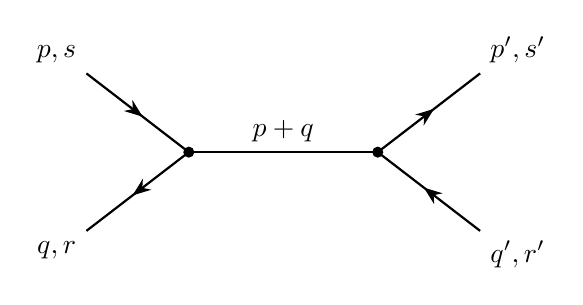
\begin{tikzpicture}[thick,
          fermion/.style={postaction={decorate},
            decoration={markings, mark=at position 0.55 with {\arrow{Stealth}}}},
        ]
          \coordinate (a)  at (-1.2, 0);
          \coordinate (b)  at ( 1.2, 0);
          \coordinate (i1) at (-2.5,  1.0);
          \coordinate (i2) at (-2.5, -1.0);
          \coordinate (f1) at ( 2.5,  1.0);
          \coordinate (f2) at ( 2.5, -1.0);
          \draw[fermion] (i1) -- (a);
          \draw[fermion] (a)  -- (i2);
          \draw[fermion] (f2) -- (b);
          \draw[fermion] (b)  -- (f1);
          \draw (a) -- (b) node[midway, above] {$p+q$};
          \fill (a) circle (2pt);
          \fill (b) circle (2pt);
          \node[above left]  at (i1) {$p,s$};
          \node[below left]  at (i2) {$q,r$};
          \node[above right] at (f1) {$p',s'$};
          \node[below right] at (f2) {$q',r'$};
        \end{tikzpicture}
        }} = (-i\lambda)^2[\bar{v}^r(\mathbf{q})u^s(\mathbf{p})]\frac{i}{(p+q)^2-\mu^2+i\epsilon}[\bar{u}^{s'}(\mathbf{p}')v^{r'}(\mathbf{q}')].
    \end{equation}
    The relative minus sign between the two channels arises from the anticommutation of the fermionic operators when bringing the $u$-channel contraction into normal order. In particular, the $t-$channel diagram is given by
    \begin{equation}
        \sim \wick{
            \c1\psi(x_1)\c1{\bar\psi}(x)}
            \wick{
            \c2{\psi}(x)
            \c2{\bar\psi}(x_3)}
            \wick{\c3\psi(y)
            \c3{\bar\psi}(x_2)}
            \wick{\c3\psi(x_4)
            \c3{\bar\psi}(y)}
            \wick{
            \c4\phi(x)\c4\phi(y)}.
    \end{equation}
    Whereas, for $s$-channel, we have
    \begin{equation}
        \sim \wick{
            \c1\psi(x_1)\c1{\bar\psi}(x)}
            \wick{
            \c2{\psi}(x)
            \c2{\bar\psi}(x_2)}
            \wick{\c3\psi(y)
            \c3{\bar\psi}(x_3)}
            \wick{\c3\psi(x_4)
            \c3{\bar\psi}(y)}
            \wick{
            \c4\phi(x)\c4\phi(y)}.
    \end{equation}
    Note that we need to anticommute three times to go from $t$- to $s$-channel, which gives an extra minus sign.
    Therefore, the total amplitude is
    \begin{equation}
        \mathcal{M} = -(-i\lambda)^2\left(\frac{[\bar{u}^{s'}(\mathbf{p}')\cdot u^s(\mathbf{p})]\,[\bar{v}^r(\mathbf{q})\cdot v^{r'}(\mathbf{q}')]}{(p-p')^2-\mu^2} - \frac{[\bar{v}^r(\mathbf{q})\cdot u^s(\mathbf{p})]\,[\bar{u}^{s'}(\mathbf{p}')\cdot v^{r'}(\mathbf{q}')]}{(p+q)^2-\mu^2}\right).
    \end{equation}
\end{solution}

\subsection{Pseudoscalar Yukawa Theory, Q5}

The Lagrangian for a pseudoscalar Yukawa interaction is given by
\begin{equation}
    \mathcal{L} = \tfrac{1}{2}(\partial\phi)^2 - \tfrac{1}{2}\mu^2\phi^2 + \bar\psi(i\slashed{\partial}-m)\psi - \lambda\phi\bar\psi\gamma^5\psi.
\end{equation}
Write down the Feynman rules for this theory. Use this to write down the amplitude at order $\lambda^2$ for $\psi\psi\to\psi\psi$ scattering and $\psi\bar\psi\to\psi\bar\psi$ scattering.

\begin{solution}
    There is not much of difference between the Feynman rules for Yukawa theory and the pseudoscalar Yukawa theory. In particular, they differ by a $\gamma^5$ at each vertex. Therefore, we can easily write down the scattering amplitude. For $\psi\psi\to\psi\psi$, we find
    \begin{equation}
        \mathcal{M} = (-i\lambda)^2\left(\frac{[\bar{u}^{s'}(\mathbf{p}')\gamma^5 u^s(\mathbf{p})]\,[\bar{u}^{r'}(\mathbf{q}')\gamma^5 u^r(\mathbf{q})]}{(p'-p)^2-\mu^2} - \frac{[\bar{u}^{s'}(\mathbf{p}')\gamma^5 u^r(\mathbf{q})]\,[\bar{u}^{r'}(\mathbf{q}')\gamma^5 u^s(\mathbf{p})]}{(q'-p)^2-\mu^2}\right).
    \end{equation}
    For $\psi\bar\psi\to\psi\bar\psi$, we have
    \begin{equation}
        \mathcal{M} = -(-i\lambda)^2\left(\frac{[\bar{u}^{s'}(\mathbf{p}') \gamma^5u^s(\mathbf{p})]\,[\bar{v}^r(\mathbf{q})\gamma^5 v^{r'}(\mathbf{q}')]}{(p-p')^2-\mu^2} - \frac{[\bar{v}^r(\mathbf{q})\gamma^5 u^s(\mathbf{p})]\,[\bar{u}^{s'}(\mathbf{p}')\gamma^5 v^{r'}(\mathbf{q}')]}{(p+q)^2-\mu^2}\right).
    \end{equation}
\end{solution}


\subsection{Compton Scattering in QED, Q7}

Consider the Compton scattering process $e^-\gamma\to e^-\gamma$ in QED. Let the incoming photon have polarization vector $\epsilon^\mu_{\rm in}$, and the outgoing photon have polarization vector $\epsilon^\mu_{\rm out}$. Use the Feynman rules to derive the following amplitude associated to the lowest order diagram,
\begin{equation}
    \vcenter{\hbox{
    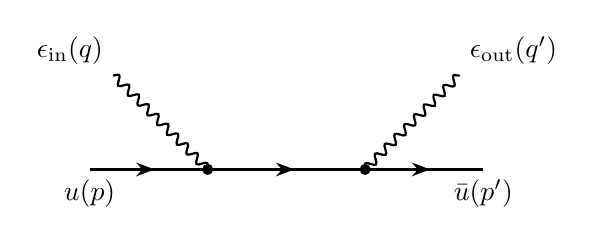
\begin{tikzpicture}[thick,
      fermion/.style={postaction={decorate},
        decoration={markings, mark=at position 0.55 with {\arrow{Stealth}}}},
      photon/.style={decorate,
        decoration={snake, amplitude=1.5pt, segment length=5pt}},
    ]
      \coordinate (v1) at (0,0);
      \coordinate (v2) at (2,0);
      \draw[fermion] (-1.5,0) -- (v1);
      \draw[fermion] (v1) -- (v2);
      \draw[fermion] (v2) -- (3.5,0);
      \draw[photon]  (-1.2,1.2) -- (v1);
      \draw[photon]  (v2) -- (3.2,1.2);
      \fill (v1) circle (2pt);
      \fill (v2) circle (2pt);
      \node[below] at (-1.5,0)   {$u(p)$};
      \node[below] at (3.5,0)    {$\bar{u}(p')$};
      \node[above left]  at (-1.2,1.2) {$\epsilon_{\rm in}(q)$};
      \node[above right] at (3.2,1.2)  {$\epsilon_{\rm out}(q')$};
    \end{tikzpicture}
    }} = (-ie)^2\bar{u}^{r'}(\mathbf{p}')\,\slashed{\epsilon}_{\rm out}\,\frac{(\slashed{p}+\slashed{q}+m)}{(p+q)^2-m^2}\,\slashed{\epsilon}_{\rm in}\,u^s(\mathbf{p}).
\end{equation}
Compute also the contribution from the diagram
\begin{equation}
    \vcenter{\hbox{
    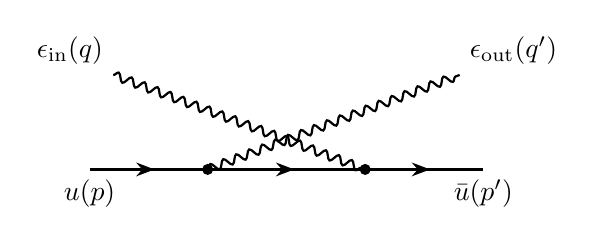
\begin{tikzpicture}[thick,
      fermion/.style={postaction={decorate},
        decoration={markings, mark=at position 0.55 with {\arrow{Stealth}}}},
      photon/.style={decorate,
        decoration={snake, amplitude=1.5pt, segment length=5pt}},
    ]
      \coordinate (v1) at (0,0);
      \coordinate (v2) at (2,0);
      \draw[fermion] (-1.5,0) -- (v1);
      \draw[fermion] (v1) -- (v2);
      \draw[fermion] (v2) -- (3.5,0);
      \draw[photon]  (-1.2,1.2) -- (v2);
      \draw[photon]  (v1) -- (3.2,1.2);
      \fill (v1) circle (2pt);
      \fill (v2) circle (2pt);
      \node[below] at (-1.5,0)   {$u(p)$};
      \node[below] at (3.5,0)    {$\bar{u}(p')$};
      \node[above left]  at (-1.2,1.2) {$\epsilon_{\rm in}(q)$};
      \node[above right] at (3.2,1.2)  {$\epsilon_{\rm out}(q')$};
    \end{tikzpicture}
    }}.
\end{equation}
The complete amplitude at order $e^2$ is the sum of these two contributions. Show that the total amplitude vanishes if $\epsilon_{\rm in}$ is replaced by the incoming photon momentum $q$. Check that the same holds true if $\epsilon_{\rm out}$ is replaced by $q'$. (Note that it will be helpful to recall the equation $(\slashed{p}-m)u(\mathbf{p})=0$ satisfied by the spinor).

\begin{solution}
    The first amplitue is given by
    \begin{equation}
        i\mathcal{M}_1 = (-ie)^2  \bar u^{r'}(\mathbf{p}')\gamma_\nu \epsilon _\text{out}^\nu\frac{i(\slashed{p}+\slashed{q}+m)}{(p+q)^2-m^2}\epsilon _\text{in}^\mu \gamma_\mu u^s(\mathbf{p}) = (-ie)^2\bar{u}^{r'}(\mathbf{p}')\,\slashed{\epsilon}_{\rm out}\,\frac{i(\slashed{p}+\slashed{q}+m)}{(p+q)^2-m^2}\,\slashed{\epsilon}_{\rm in}\,u^s(\mathbf{p}).
    \end{equation}
    Similarly, the second amplitude is given by
    \begin{equation}
        i\mathcal{M}_2 = (-ie)^2\bar{u}^{r'}(\mathbf{p}')\,\slashed{\epsilon}_{\rm in}\,\frac{i(\slashed{p}-\slashed{q}'+m)}{(p-q   ')^2-m^2}\,\slashed{\epsilon}_{\rm out}\,u^s(\mathbf{p}).
    \end{equation}
    Therefore, the total amplitude is given by
    \begin{equation}
        \mathcal{M} = (-ie)^2\bar{u}^{r'}(\mathbf{p}')\left[\slashed{\epsilon}_{\rm out}\,\frac{\slashed{p}+\slashed{q}+m}{(p+q)^2-m^2}\,\slashed{\epsilon}_{\rm in} + \slashed{\epsilon}_{\rm in}\,\frac{\slashed{p}-\slashed{q}'+m}{(p-q')^2-m^2}\,\slashed{\epsilon}_{\rm out}\right]u^s(\mathbf{p}).
    \end{equation}
    Replace $\epsilon_{\rm in}$ by $q$, and use momentum conservation, we find
    \begin{equation}
    \begin{aligned}
        \mathcal{M} &= (-ie)^2\bar{u}^{r'}(\mathbf{p}')\left[\slashed{\epsilon}_{\rm out}\,\frac{\slashed{p}+\slashed{q}+m}{(p+q)^2-m^2}\,\slashed{q} + \slashed{q}\,\frac{\slashed{p}-\slashed{q}'+m}{(p-q')^2-m^2}\,\slashed{\epsilon}_{\rm out}\right]u^s(\mathbf{p}).
    \end{aligned}
    \end{equation}
    Using 
    \begin{equation}
        \slashed{p}\slashed{q} = -\slashed{q}\slashed{p} +2p\cdot q, \quad {\rm and} \quad \slashed{q}^2 = q^2 = 0,
    \end{equation}
    the first term becomes
    \begin{equation}
        (-ie)^2\bar{u}^{r'}(\mathbf{p}') \slashed{q}\frac{-\slashed{p}+m}{(p+q)^2-m^2}u^s(\mathbf{p}) = 0
    \end{equation}
    by $(\slashed{p}-m)u(\mathbf{p})=0$. Similarly, the second term also vanishes. Therefore, we have verified the Ward identity to tree level for Compton Scattering.
\end{solution}

\subsection{QED Amplitude for \texorpdfstring{$e^-e^+\to\mu^-\mu^+$}{e+e- to mu+mu-}, Q8}

Use the Feynman rules to show that the QED amplitude for $e^-e^+\to\mu^-\mu^+$ is given at lowest order in $e$ by,
\begin{equation}
    \vcenter{\hbox{
    \begin{tikzpicture}[thick,
      every node/.style={font=\small},
      fermion/.style={postaction={decorate},
        decoration={markings, mark=at position 0.55 with {\arrow{Stealth[length=2.2mm]}}}},
      antifermion/.style={postaction={decorate},
        decoration={markings, mark=at position 0.55 with {\arrowreversed{Stealth[length=2.2mm]}}}},
      photon/.style={decorate,
        decoration={snake, amplitude=1.5pt, segment length=5pt}},
      mom/.style={-{Stealth[length=2mm]}, thin},
    ]
      \coordinate (a)   at (0,   0);
      \coordinate (b)   at (3.0, 0);
      \coordinate (em)  at (-2.0,  1.4);
      \coordinate (ep)  at (-2.0, -1.4);
      \coordinate (mum) at ( 5.0,  1.4);
      \coordinate (mup) at ( 5.0, -1.4);
    
      \draw[fermion]     (em)  -- (a);
      \draw[antifermion] (ep)  -- (a);
      \draw[photon]      (a)   -- (b);
      \draw[fermion]     (b)   -- (mum);
      \draw[antifermion] (b)   -- (mup);
    
      \draw[mom] ($(em)!0.2!(a)!0.25cm!90:(a)$)   -- ($(em)!0.8!(a)!0.25cm!90:(a)$)
        node[midway, above=6pt,  inner sep=1pt] {$p,s$};
      \draw[mom]  ($(a)!0.8!(ep)!0.25cm!90:(ep)$) -- ($(a)!0.2!(ep)!0.25cm!90:(ep)$) 
        node[midway, below=6pt,  inner sep=1pt] {$q,r$};
      \draw[mom] ($(a)!0.2!(b) +(0,0.30)$)        -- ($(a)!0.8!(b) +(0,0.30)$)
        node[midway, above] {$p{+}q$};
      \draw[mom] ($(b)!0.2!(mum)!0.25cm!90:(mum)$) -- ($(b)!0.8!(mum)!0.25cm!90:(mum)$)
        node[midway, above=6pt, inner sep=1pt] {$p',s'$};
      \draw[mom] ($(mup)!0.8!(b)!0.25cm!90:(b)$) -- ($(mup)!0.2!(b)!0.25cm!90:(b)$)
        node[midway, below=6pt, inner sep=1pt] {$q',r'$};
    
      \node[left]  at (em)  {$e^-$};
      \node[left]  at (ep)  {$e^+$};
      \node[right] at (mum) {$\mu^-$};
      \node[right] at (mup) {$\mu^+$};
    \end{tikzpicture}
    }} = (-ie)^2\,\frac{[\bar{v}_e^r(\mathbf{q})\,\gamma_\mu\, u_e^s(\mathbf{p})]\,[\bar{u}_m^{s'}(\mathbf{p}')\,\gamma^\mu\, v_m^{r'}(\mathbf{q}')]}{(p+q)^2}
\end{equation}
where the subscripts $e$ and $m$ denote whether the spinors satisfy the Dirac equation for electrons or for muons.

\begin{solution}
    This can be trivially seen using the momentum space Feynman rules.
\end{solution}

\subsection{Pair Creation of Scalar Particles by Photons, Q9}

Viki Weisskopf is one of the more charming characters from the history of quantum field theory. This is from his autobiography:

\begin{quote}
    ``Pauli asked me to calculate the amplitude for pair creation of scalar particles by photons. It was only a short time after Bethe and Heitler had solved the same problem for electrons and positrons. I met Bethe in Copenhagen at a conference and asked him to tell me how he did the calculations. I also inquired how long it would take to perform this task; he answered, `It would take me three days, but you will need about three weeks.' He was right, as usual; furthermore, the published result was wrong by a factor of four.''
\end{quote}

Can you do better?

\begin{solution}
    The scalar QED has the Lagrangian
    \begin{equation}
        \mathcal{L}= |D\phi|^2 - m^2|\phi|^2 -\frac{1}{4}F_{\mu\nu}F^{\mu\nu} = |\partial\phi|^2 - m^2|\phi|^2 -\frac{1}{4}F_{\mu\nu}F^{\mu\nu} +ieA^\mu(\phi\partial_\mu\phi^*-\phi^*\partial_\mu\phi)-e^2A_\mu A^\mu|\phi|^2.
    \end{equation}
    The corresponding Feynman rules are considerably more complicated. The propagators are just the normal scalar and photon propagators. However, there are two types of vertices, and one involves the derivative of the fields. Consider a three-point vertex, for example, that annihilates a particle with momentum $p$ and an antiparticle with momentum $p'$. Then, the derivative of $\phi$ only acts on the $a_\mathbf{p}$ term, giving a factor of $-ip_\mu$. Similarly, the derivative on $\phi^*$ only acts on the $b_\mathbf{p}$ term, giving a factor of $-ip'_\mu$. Therefore, one could conclude that for arrow flow pointing to the right, we obtain a factor of $-p_\mu$; for every arrow flow pointing to the left at a vertex, we obtain a factor of $+p_\mu$ (remember the extra $i$ from the perturbative expansion of Dyson's equation).

    Therefore, the vertex rules are

    \begin{equation}
        \vcenter{\hbox{
        \begin{tikzpicture}[thick,
          cscalar/.style={dashed, postaction={decorate},
            decoration={markings, mark=at position 0.55 with {\arrow{Stealth[length=2.2mm]}}}},
          antiscalar/.style={dashed, postaction={decorate},
            decoration={markings, mark=at position 0.55 with {\arrowreversed{Stealth[length=2.2mm]}}}},
          photon/.style={decorate,
            decoration={snake, amplitude=1.2mm, segment length=2.5mm}},
          mom arrow/.style={-{Stealth[length=2.2mm]}, thin},
        ]
          \coordinate (v)   at ( 0,    0);
          \coordinate (i1)  at (-1.5,  1.0);
          \coordinate (i2)  at (-1.5, -1.0);
          \coordinate (f1)  at ( 1.5,  0.0);
          \draw[cscalar]    (i1) -- (v);   % phi incoming, particle arrow inward
          \draw[cscalar] (v)  -- (i2);  % phi* incoming, antiparticle arrow outward
          \draw[photon]     (v)  -- (f1);
          % momentum arrows, both pointing INTO vertex
          \draw[mom arrow]
            ($(i1)!0.2!(v)!0.25cm!90:(v)$) -- ($(i1)!0.8!(v)!0.25cm!90:(v)$)
            node[midway, above=3pt, inner sep=1pt] {$p$};
          \draw[mom arrow]
            ($(i2)!0.2!(v)!-0.25cm!90:(v)$) -- ($(i2)!0.8!(v)!-0.25cm!90:(v)$)
            node[midway, below=3pt, inner sep=1pt] {$p'$};
          \node[left]  at (i1) {$\phi$};
          \node[left]  at (i2) {$\phi^*$};
          \node[right] at (f1) {$A^\mu$};
        \end{tikzpicture}
        }} = -ie(-p + p')^\mu,
    \end{equation}
    and

    \begin{equation}
        \vcenter{\hbox{
        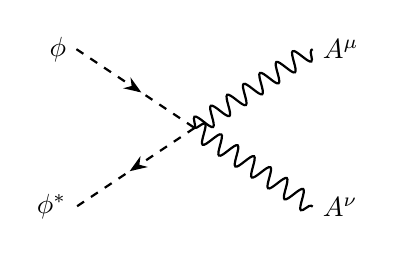
\begin{tikzpicture}[thick,
          cscalar/.style={dashed, postaction={decorate},
            decoration={markings, mark=at position 0.55 with {\arrow{Stealth[length=2.2mm]}}}},
          antiscalar/.style={dashed, postaction={decorate},
            decoration={markings, mark=at position 0.55 with {\arrowreversed{Stealth[length=2.2mm]}}}},
          photon/.style={decorate,
            decoration={snake, amplitude=1.2mm, segment length=2.5mm}},
        ]
          \coordinate (v)   at ( 0,    0);
          \coordinate (i1)  at (-1.5,  1.0);
          \coordinate (i2)  at (-1.5, -1.0);
          \coordinate (f1)  at ( 1.5,  1.0);
          \coordinate (f2)  at ( 1.5, -1.0);
          \draw[cscalar]    (i1) -- (v);
          \draw[cscalar] (v)  -- (i2);
          \draw[photon]     (v)  -- (f1);
          \draw[photon]     (v)  -- (f2);
          \node[left]  at (i1) {$\phi$};
          \node[left]  at (i2) {$\phi^*$};
          \node[right] at (f1) {$A^\mu$};
          \node[right] at (f2) {$A^\nu$};
        \end{tikzpicture}
        }} = 2ie^2\eta^{\mu\nu}.
    \end{equation}

    For pair creation, three diagrams contribute at the tree level to first order:
    
    \begin{tikzpicture}[thick, scale=0.7,
      every node/.style={font=\small},
      cscalar/.style={dashed, postaction={decorate},
        decoration={markings, mark=at position 0.55 with {\arrow{Stealth[length=2mm]}}}},
      antiscalar/.style={dashed, postaction={decorate},
        decoration={markings, mark=at position 0.55 with {\arrowreversed{Stealth[length=2mm]}}}},
      photon/.style={decorate,
        decoration={snake, amplitude=1.2mm, segment length=2.5mm}},
      mom/.style={-{Stealth[length=2mm]}, thin},
    ]
    \centering{
    % t-channel
    \coordinate (a) at (0, 1.5); \coordinate (b) at (0,-1.5);
    \coordinate (k1in) at (-2.5,1.5); \coordinate (k2in) at (-2.5,-1.5);
    \coordinate (pmout) at (2.5,1.5); \coordinate (ppout) at (2.5,-1.5);
    \draw[photon] (k1in)--(a); \draw[photon] (k2in)--(b);
    \draw[cscalar] (a)--(b) node[midway,right=4pt]{$k_1{-}p$};
    \draw[cscalar] (a)--(pmout); \draw[antiscalar] (b)--(ppout);
    \draw[mom] ($(k1in)!0.2!(a)+(0,.28)$)--($(k1in)!0.8!(a)+(0,.28)$) node[midway,above]{$k_1$};
    \draw[mom] ($(k2in)!0.2!(b)+(0,-.28)$)--($(k2in)!0.8!(b)+(0,-.28)$) node[midway,below]{$k_2$};
    \draw[mom] ($(a)!0.2!(pmout)+(0,.28)$)--($(a)!0.8!(pmout)+(0,.28)$) node[midway,above]{$p$};
    \draw[mom] ($(b)!0.2!(ppout)+(0,-.28)$)--($(b)!0.8!(ppout)+(0,-.28)$) node[midway,below]{$q$};
    \node[left] at (k1in){$\gamma$}; \node[left] at (k2in){$\gamma$};
    \node[right] at (pmout){$\phi$}; \node[right] at (ppout){$\phi^*$};
    \node[below] at (0,-2.5){$t$-channel};
    
    % u-channel
    \begin{scope}[xshift=7.5cm]
    \coordinate (a) at (0,1.5); \coordinate (b) at (0,-1.5);
    \coordinate (k1in) at (-2.5,1.5); \coordinate (k2in) at (-2.5,-1.5);
    \coordinate (ppout) at (2.5,1.5); \coordinate (pmout) at (2.5,-1.5);
    \draw[photon] (k1in)--(a); \draw[photon] (k2in)--(b);
    \draw[cscalar] (a)--(b) node[midway,right=4pt]{$k_1{-}q$};
    \draw[antiscalar] (a)--(ppout); \draw[cscalar] (b)--(pmout);
    \draw[mom] ($(k1in)!0.2!(a)+(0,.28)$)--($(k1in)!0.8!(a)+(0,.28)$) node[midway,above]{$k_1$};
    \draw[mom] ($(k2in)!0.2!(b)+(0,-.28)$)--($(k2in)!0.8!(b)+(0,-.28)$) node[midway,below]{$k_2$};
    \draw[mom] ($(a)!0.2!(ppout)+(0,.28)$)--($(a)!0.8!(ppout)+(0,.28)$) node[midway,above]{$q$};
    \draw[mom] ($(b)!0.2!(pmout)+(0,-.28)$)--($(b)!0.8!(pmout)+(0,-.28)$) node[midway,below]{$p$};
    \node[left] at (k1in){$\gamma$}; \node[left] at (k2in){$\gamma$};
    \node[right] at (ppout){$\phi^*$}; \node[right] at (pmout){$\phi$};
    \node[below] at (0,-2.5){$u$-channel};
    \end{scope}
    
    % seagull
    \begin{scope}[xshift=15cm]
    \coordinate (v) at (0,0);
    \coordinate (k1in) at (-2.5,1.2); \coordinate (k2in) at (-2.5,-1.2);
    \coordinate (pmout) at (2.5,1.2); \coordinate (ppout) at (2.5,-1.2);
    \draw[photon] (k1in)--(v); \draw[photon] (k2in)--(v);
    \draw[cscalar] (v)--(pmout); \draw[antiscalar] (v)--(ppout);
    \draw[mom] ($(k1in)!0.2!(v)+(0,.28)$)--($(k1in)!0.8!(v)+(0,.28)$) node[midway,above]{$k_1$};
    \draw[mom] ($(k2in)!0.2!(v)+(0,-.28)$)--($(k2in)!0.8!(v)+(0,-.28)$) node[midway,below]{$k_2$};
    \draw[mom] ($(v)!0.2!(pmout)+(0,.28)$)--($(v)!0.8!(pmout)+(0,.28)$) node[midway,above]{$p$};
    \draw[mom] ($(v)!0.2!(ppout)+(0,-.28)$)--($(v)!0.8!(ppout)+(0,-.28)$) node[midway,below]{$q$};
    \node[left] at (k1in){$\gamma$}; \node[left] at (k2in){$\gamma$};
    \node[right] at (pmout){$\phi$}; \node[right] at (ppout){$\phi^*$};
    \node[below] at (0,-2.5){seagull};
    \end{scope}}
    \end{tikzpicture}
    
    The $t$-channel has amplitude
    \begin{equation}
    \begin{aligned}
        i\mathcal{M}_t &= -(-ie)^2\epsilon_\nu^2[-q^\nu +(k_1^\nu-p^\nu)]\frac{i}{(k_1-p)^2-m^2}\epsilon_\mu^1[-p^\mu-(k_1^\mu-p^\mu)]\\
        &=-(-ie)^2(\epsilon_2\cdot k_2)\frac{i}{(k_1-p)^2-m^2}(\epsilon_1\cdot k_1).
    \end{aligned}
    \end{equation}
    For the $u$-channel, we simply get
    \begin{equation}
        i\mathcal{M}_u = -(-ie)^2(\epsilon_2\cdot k_2)\frac{i}{(k_1-q)^2-m^2}(\epsilon_1\cdot k_1).
    \end{equation}
    Finally, the seagull diagram gives
    \begin{equation}
        i\mathcal{M}_4 = 2ie^2(\epsilon_1\cdot\epsilon_2).
    \end{equation}
    Therefore, the total amplitude is 
    \begin{equation}
        \mathcal{M} = e^2(\epsilon_2\cdot k_2)\left[\frac{1}{(k_1-q)^2-m^2} + \frac{1}{(k_1-p)^2-m^2}\right](\epsilon_1\cdot k_1) +2e^2(\epsilon_1\cdot\epsilon_2).
    \end{equation}
\end{solution}